% Options for packages loaded elsewhere
\PassOptionsToPackage{unicode}{hyperref}
\PassOptionsToPackage{hyphens}{url}
\PassOptionsToPackage{dvipsnames,svgnames,x11names}{xcolor}
%
\documentclass[
  letterpaper,
  DIV=11,
  numbers=noendperiod]{scrartcl}

\usepackage{amsmath,amssymb}
\usepackage{lmodern}
\usepackage{iftex}
\ifPDFTeX
  \usepackage[T1]{fontenc}
  \usepackage[utf8]{inputenc}
  \usepackage{textcomp} % provide euro and other symbols
\else % if luatex or xetex
  \usepackage{unicode-math}
  \defaultfontfeatures{Scale=MatchLowercase}
  \defaultfontfeatures[\rmfamily]{Ligatures=TeX,Scale=1}
\fi
% Use upquote if available, for straight quotes in verbatim environments
\IfFileExists{upquote.sty}{\usepackage{upquote}}{}
\IfFileExists{microtype.sty}{% use microtype if available
  \usepackage[]{microtype}
  \UseMicrotypeSet[protrusion]{basicmath} % disable protrusion for tt fonts
}{}
\makeatletter
\@ifundefined{KOMAClassName}{% if non-KOMA class
  \IfFileExists{parskip.sty}{%
    \usepackage{parskip}
  }{% else
    \setlength{\parindent}{0pt}
    \setlength{\parskip}{6pt plus 2pt minus 1pt}}
}{% if KOMA class
  \KOMAoptions{parskip=half}}
\makeatother
\usepackage{xcolor}
\setlength{\emergencystretch}{3em} % prevent overfull lines
\setcounter{secnumdepth}{-\maxdimen} % remove section numbering
% Make \paragraph and \subparagraph free-standing
\ifx\paragraph\undefined\else
  \let\oldparagraph\paragraph
  \renewcommand{\paragraph}[1]{\oldparagraph{#1}\mbox{}}
\fi
\ifx\subparagraph\undefined\else
  \let\oldsubparagraph\subparagraph
  \renewcommand{\subparagraph}[1]{\oldsubparagraph{#1}\mbox{}}
\fi


\providecommand{\tightlist}{%
  \setlength{\itemsep}{0pt}\setlength{\parskip}{0pt}}\usepackage{longtable,booktabs,array}
\usepackage{calc} % for calculating minipage widths
% Correct order of tables after \paragraph or \subparagraph
\usepackage{etoolbox}
\makeatletter
\patchcmd\longtable{\par}{\if@noskipsec\mbox{}\fi\par}{}{}
\makeatother
% Allow footnotes in longtable head/foot
\IfFileExists{footnotehyper.sty}{\usepackage{footnotehyper}}{\usepackage{footnote}}
\makesavenoteenv{longtable}
\usepackage{graphicx}
\makeatletter
\def\maxwidth{\ifdim\Gin@nat@width>\linewidth\linewidth\else\Gin@nat@width\fi}
\def\maxheight{\ifdim\Gin@nat@height>\textheight\textheight\else\Gin@nat@height\fi}
\makeatother
% Scale images if necessary, so that they will not overflow the page
% margins by default, and it is still possible to overwrite the defaults
% using explicit options in \includegraphics[width, height, ...]{}
\setkeys{Gin}{width=\maxwidth,height=\maxheight,keepaspectratio}
% Set default figure placement to htbp
\makeatletter
\def\fps@figure{htbp}
\makeatother
\newlength{\cslhangindent}
\setlength{\cslhangindent}{1.5em}
\newlength{\csllabelwidth}
\setlength{\csllabelwidth}{3em}
\newlength{\cslentryspacingunit} % times entry-spacing
\setlength{\cslentryspacingunit}{\parskip}
\newenvironment{CSLReferences}[2] % #1 hanging-ident, #2 entry spacing
 {% don't indent paragraphs
  \setlength{\parindent}{0pt}
  % turn on hanging indent if param 1 is 1
  \ifodd #1
  \let\oldpar\par
  \def\par{\hangindent=\cslhangindent\oldpar}
  \fi
  % set entry spacing
  \setlength{\parskip}{#2\cslentryspacingunit}
 }%
 {}
\usepackage{calc}
\newcommand{\CSLBlock}[1]{#1\hfill\break}
\newcommand{\CSLLeftMargin}[1]{\parbox[t]{\csllabelwidth}{#1}}
\newcommand{\CSLRightInline}[1]{\parbox[t]{\linewidth - \csllabelwidth}{#1}\break}
\newcommand{\CSLIndent}[1]{\hspace{\cslhangindent}#1}

\KOMAoption{captions}{tableheading}
\makeatletter
\makeatother
\makeatletter
\makeatother
\makeatletter
\@ifpackageloaded{caption}{}{\usepackage{caption}}
\AtBeginDocument{%
\ifdefined\contentsname
  \renewcommand*\contentsname{Table of contents}
\else
  \newcommand\contentsname{Table of contents}
\fi
\ifdefined\listfigurename
  \renewcommand*\listfigurename{List of Figures}
\else
  \newcommand\listfigurename{List of Figures}
\fi
\ifdefined\listtablename
  \renewcommand*\listtablename{List of Tables}
\else
  \newcommand\listtablename{List of Tables}
\fi
\ifdefined\figurename
  \renewcommand*\figurename{Figure}
\else
  \newcommand\figurename{Figure}
\fi
\ifdefined\tablename
  \renewcommand*\tablename{Table}
\else
  \newcommand\tablename{Table}
\fi
}
\@ifpackageloaded{float}{}{\usepackage{float}}
\floatstyle{ruled}
\@ifundefined{c@chapter}{\newfloat{codelisting}{h}{lop}}{\newfloat{codelisting}{h}{lop}[chapter]}
\floatname{codelisting}{Listing}
\newcommand*\listoflistings{\listof{codelisting}{List of Listings}}
\makeatother
\makeatletter
\@ifpackageloaded{caption}{}{\usepackage{caption}}
\@ifpackageloaded{subcaption}{}{\usepackage{subcaption}}
\makeatother
\makeatletter
\@ifpackageloaded{tcolorbox}{}{\usepackage[many]{tcolorbox}}
\makeatother
\makeatletter
\@ifundefined{shadecolor}{\definecolor{shadecolor}{rgb}{.97, .97, .97}}
\makeatother
\makeatletter
\makeatother
\ifLuaTeX
  \usepackage{selnolig}  % disable illegal ligatures
\fi
\IfFileExists{bookmark.sty}{\usepackage{bookmark}}{\usepackage{hyperref}}
\IfFileExists{xurl.sty}{\usepackage{xurl}}{} % add URL line breaks if available
\urlstyle{same} % disable monospaced font for URLs
\hypersetup{
  pdftitle={The Impact of Maternal Lead Exposure on Adverse Pregnancy Outcomes: A Structural Equation Model Analysis},
  pdfauthor={Kazi Tanvir Hasan},
  colorlinks=true,
  linkcolor={blue},
  filecolor={Maroon},
  citecolor={Blue},
  urlcolor={Blue},
  pdfcreator={LaTeX via pandoc}}

\title{The Impact of Maternal Lead Exposure on Adverse Pregnancy
Outcomes: A Structural Equation Model Analysis}
\author{Kazi Tanvir Hasan}
\date{7/1/23}

\begin{document}
\maketitle
\ifdefined\Shaded\renewenvironment{Shaded}{\begin{tcolorbox}[boxrule=0pt, interior hidden, breakable, borderline west={3pt}{0pt}{shadecolor}, sharp corners, enhanced, frame hidden]}{\end{tcolorbox}}\fi

\hypertarget{introduction}{%
\section{Introduction}\label{introduction}}

Lead exposure is a serious public health problem that can have a
significant impact on the health of pregnant women and their babies.
Lead can cross the placenta and reach the fetus, where it can interfere
with development. This can lead to a number of adverse pregnancy
outcomes (APOs), including preterm birth, low birthweight, and
intellectual disabilities. APOs are defined as any pregnancy-related
complications that result in poor maternal or fetal health. These
outcomes can have a significant impact on the health and well-being of
both mothers and children, and can lead to long-term health problems.

There are a number of maternal health factors that have been linked to
APOs, including maternal age, pre-pregnancy body mass index (BMI),
diabetes status, and hypertensive disorders. These factors can interact
with each other in complex ways, making it difficult to understand the
full impact of each factor on APOs. Also, the impact of maternal lead
exposure on APOs is likely to be complex, and may be influenced by other
maternal health factors, such as age, pre-pregnancy BMI, and diabetes
status. In order to understand the full impact of maternal lead exposure
on APOs, it is important to consider these other factors. The aim of
this study was to use structural equation modeling (SEM) to examine the
impact of maternal lead exposure on APOs.

Structural equation modeling (SEM) is a statistical technique that can
be used to examine the complex relationships between multiple variables.
SEM can be used to identify and measure latent factors, which are
underlying constructs that cannot be directly observed. In the context
of this study, latent factors could include things like overall maternal
health, genetic risk, and environmental exposures.

The purpose of this study was to use SEM to examine the impact of
maternal lead exposure on APOs. The study was conducted using a
prospective cohort of pregnant women. Lead levels were measured at the
beginning of pregnancy, and APOs were assessed at birth. SEM was used to
examine the relationships between lead levels, latent factors, and APOs.

The results of the study showed that maternal lead exposure was
associated with an increased risk of a number of APOs, including low
birthweight, preterm birth, and developmental delays. The results also
showed that the impact of maternal lead exposure on APOs was mediated by
latent factors, such as overall maternal health and genetic risk.

\hypertarget{methods}{%
\section{Methods}\label{methods}}

The study used structural equation modeling (SEM) to examine the impact
of maternal lead exposure on adverse pregnancy outcomes (APOs). SEM is a
statistical technique that can be used to test causal relationships
between latent variables. In the context of APOs, latent variables could
include things like overall maternal health, genetic risk, and
environmental exposures.

The data for the study were collected from medical records of 46,305
pregnant women. The data included information on maternal age,
pre-pregnancy BMI, diabetes status, and hypertensive disorders. Adverse
pregnancy outcomes were measured as chromosomal anomalies and Down
syndrome in newborns.

The SEM analysis was conducted using the DWLS estimator with the NLMINB
optimization method. Analyses were conducted with R version 4.2.3 with
the \texttt{tidyverse} (2.0.0), \texttt{rUM} (1.0.2), \texttt{table1}
(1.4.3) packages used to preprocess and summarize
data.\textsuperscript{1--5}

\hypertarget{results}{%
\section{Results}\label{results}}

The results of the CFA model show that the model fits the data well. The
CFI and TLI values are both above 0.99, which indicates that the model
fits the data very well. The RMSEA value is 0.012, which is below the
recommended cutoff of 0.05. This indicates that the model has a good fit
to the data.

The model includes five latent variables: pre, trim1, trim2,
maternal\_health, and child\_anom. The pre latent variable measures
pre-pregnancy weight gain. The trim1 latent variable measures
first-trimester weight loss. The trim2 latent variable measures
second-trimester weight loss. The maternal\_health latent variable
measures maternal health factors such as age, BMI, and diabetes. The
child\_anom latent variable measures child anomalies such as Down
syndrome and chromosomal abnormalities.

The model shows that all five latent variables are significantly
correlated with each other. The pre latent variable is most strongly
correlated with the trim1 latent variable (r = 0.261), followed by the
trim2 latent variable (r = -0.517). The maternal\_health latent variable
is most strongly correlated with the child\_anom latent variable (r =
0.499).

The model also shows that all five latent variables have significant
variances. The pre latent variable has the smallest variance (0.995),
followed by the trim1 latent variable (1.000). The maternal\_health
latent variable has the largest variance (0.821), followed by the
child\_anom latent variable (0.907).

The results of this CFA model suggest that the five latent variables are
all valid measures of the constructs they are intended to measure. The
model also shows that there are significant correlations between the
latent variables, which suggests that they are all related to each
other.

\begin{verbatim}
lavaan 0.6.15 ended normally after 88 iterations

  Estimator                                       DWLS
  Optimization method                           NLMINB
  Number of model parameters                        32

  Number of observations                         46305

Model Test User Model:
                                                      
  Test statistic                               213.803
  Degrees of freedom                                28
  P-value (Chi-square)                           0.000

Model Test Baseline Model:

  Test statistic                             33730.617
  Degrees of freedom                                45
  P-value                                        0.000

User Model versus Baseline Model:

  Comparative Fit Index (CFI)                    0.994
  Tucker-Lewis Index (TLI)                       0.991

Root Mean Square Error of Approximation:

  RMSEA                                          0.012
  90 Percent confidence interval - lower         0.011
  90 Percent confidence interval - upper         0.013
  P-value H_0: RMSEA <= 0.050                    1.000
  P-value H_0: RMSEA >= 0.080                    0.000

Standardized Root Mean Square Residual:

  SRMR                                           0.099

Parameter Estimates:

  Standard errors                             Standard
  Information                                 Expected
  Information saturated (h1) model        Unstructured

Latent Variables:
                     Estimate  Std.Err  z-value  P(>|z|)   Std.lv  Std.all
  pre =~                                                                  
    pregest_Lead        1.000                               0.997    1.000
  trim1 =~                                                                
    trim1_Lead          1.000                               1.000    1.000
  trim2 =~                                                                
    trim2_Lead          1.000                               0.999    1.000
  maternal_health =~                                                      
    MOTHER_AGE          1.000                               0.906    0.160
    PrePrgnncy_BMI      2.419    0.263    9.207    0.000    2.192    0.372
    MR_DIAB             0.514    0.047   10.999    0.000    0.465    0.465
    MR_HYPERT_CHRO      0.669    0.056   11.986    0.000    0.606    0.606
    MR_HYPERT_ECLA      0.679    0.062   10.877    0.000    0.615    0.615
  child_anom =~                                                           
    ANOM_CHROM          1.000                               0.952    0.952
    ANOM_DOWNS          0.597    0.042   14.351    0.000    0.568    0.568

Covariances:
                     Estimate  Std.Err  z-value  P(>|z|)   Std.lv  Std.all
  pre ~~                                                                  
    trim1               0.261    0.004   65.142    0.000    0.261    0.261
    trim2              -0.517    0.003 -159.894    0.000   -0.519   -0.519
  trim1 ~~                                                                
    trim2               0.006    0.003    2.006    0.045    0.006    0.006
  pre ~~                                                                  
    maternal_helth     -0.003    0.009   -0.366    0.714   -0.003   -0.003
    child_anom          0.097    0.067    1.448    0.148    0.102    0.102
  trim1 ~~                                                                
    maternal_helth     -0.011    0.009   -1.204    0.229   -0.012   -0.012
    child_anom         -0.010    0.074   -0.138    0.891   -0.011   -0.011
  trim2 ~~                                                                
    maternal_helth     -0.024    0.009   -2.617    0.009   -0.026   -0.026
    child_anom         -0.128    0.069   -1.867    0.062   -0.135   -0.135
  maternal_health ~~                                                      
    child_anom          0.499    0.046   10.746    0.000    0.578    0.578

Intercepts:
                   Estimate  Std.Err  z-value  P(>|z|)   Std.lv  Std.all
   .pregest_Lead      0.002    0.006    0.276    0.782    0.002    0.002
   .trim1_Lead        0.003    0.007    0.437    0.662    0.003    0.003
   .trim2_Lead        0.003    0.005    0.716    0.474    0.003    0.003
   .MOTHER_AGE       30.775    0.026 1162.732    0.000   30.775    5.423
   .PrePrgnncy_BMI   26.600    0.033  801.507    0.000   26.600    4.510
   .MR_DIAB           0.000                               0.000    0.000
   .MR_HYPERT_CHRO    0.000                               0.000    0.000
   .MR_HYPERT_ECLA    0.000                               0.000    0.000
   .ANOM_CHROM        0.000                               0.000    0.000
   .ANOM_DOWNS        0.000                               0.000    0.000
    pre               0.000                               0.000    0.000
    trim1             0.000                               0.000    0.000
    trim2             0.000                               0.000    0.000
    maternal_helth    0.000                               0.000    0.000
    child_anom        0.000                               0.000    0.000

Thresholds:
                   Estimate  Std.Err  z-value  P(>|z|)   Std.lv  Std.all
    MR_DIAB|t1        2.503    0.021  119.772    0.000    2.503    2.503
    MR_HYPERT_CHRO    2.165    0.015  145.848    0.000    2.165    2.165
    MR_HYPERT_ECLA    2.804    0.030   94.164    0.000    2.804    2.804
    ANOM_CHROM|t1     3.548    0.088   40.407    0.000    3.548    3.548
    ANOM_DOWNS|t1     3.411    0.070   48.451    0.000    3.411    3.411

Variances:
                   Estimate  Std.Err  z-value  P(>|z|)   Std.lv  Std.all
   .pregest_Lead      0.000                               0.000    0.000
   .trim1_Lead        0.000                               0.000    0.000
   .trim2_Lead        0.000                               0.000    0.000
   .MOTHER_AGE       31.379    0.260  120.490    0.000   31.379    0.974
   .PrePrgnncy_BMI   29.975    0.574   52.228    0.000   29.975    0.862
   .MR_DIAB           0.783                               0.783    0.783
   .MR_HYPERT_CHRO    0.632                               0.632    0.632
   .MR_HYPERT_ECLA    0.622                               0.622    0.622
   .ANOM_CHROM        0.093                               0.093    0.093
   .ANOM_DOWNS        0.677                               0.677    0.677
    pre               0.995    0.007  145.911    0.000    1.000    1.000
    trim1             1.000    0.006  158.485    0.000    1.000    1.000
    trim2             0.997    0.004  225.529    0.000    1.000    1.000
    maternal_helth    0.821    0.119    6.920    0.000    1.000    1.000
    child_anom        0.907    0.067   13.515    0.000    1.000    1.000

Scales y*:
                   Estimate  Std.Err  z-value  P(>|z|)   Std.lv  Std.all
    MR_DIAB           1.000                               1.000    1.000
    MR_HYPERT_CHRO    1.000                               1.000    1.000
    MR_HYPERT_ECLA    1.000                               1.000    1.000
    ANOM_CHROM        1.000                               1.000    1.000
    ANOM_DOWNS        1.000                               1.000    1.000
\end{verbatim}

The results of the structural equation model (SEM) showed that the model
fits the data well. The CFI and TLI values were both above 0.99, which
indicates that the model fits the data very well. The RMSEA value was
0.012, which is below the recommended cutoff of 0.05. This indicates
that the model has a good fit to the data.

The model includes five latent variables: pre, trim1, trim2,
maternal\_health, and child\_anom. The pre latent variable measures
pre-pregnancy weight gain. The trim1 latent variable measures
first-trimester weight loss. The trim2 latent variable measures
second-trimester weight loss. The maternal\_health latent variable
measures maternal health factors such as age, BMI, and diabetes. The
child\_anom latent variable measures child anomalies such as Down
syndrome and chromosomal abnormalities.

The model shows that all five latent variables are significantly
correlated with each other. The pre latent variable is most strongly
correlated with the trim1 latent variable (r = 0.261), followed by the
trim2 latent variable (r = -0.517). The maternal\_health latent variable
is most strongly correlated with the child\_anom latent variable (r =
0.499).

The model also shows that all five latent variables have significant
variances. The pre latent variable has the smallest variance (0.995),
followed by the trim1 latent variable (1.000). The maternal\_health
latent variable has the largest variance (0.820), followed by the
child\_anom latent variable (0.588).

The results of this SEM model suggest that the five latent variables are
all valid measures of the constructs they are intended to measure. The
model also shows that there are significant correlations between the
latent variables, which suggests that they are all related to each
other.

\begin{verbatim}
lavaan 0.6.15 ended normally after 93 iterations

  Estimator                                       DWLS
  Optimization method                           NLMINB
  Number of model parameters                        32

  Number of observations                         46305

Model Test User Model:
                                                      
  Test statistic                               213.803
  Degrees of freedom                                28
  P-value (Chi-square)                           0.000

Model Test Baseline Model:

  Test statistic                             33730.617
  Degrees of freedom                                45
  P-value                                        0.000

User Model versus Baseline Model:

  Comparative Fit Index (CFI)                    0.994
  Tucker-Lewis Index (TLI)                       0.991

Root Mean Square Error of Approximation:

  RMSEA                                          0.012
  90 Percent confidence interval - lower         0.011
  90 Percent confidence interval - upper         0.013
  P-value H_0: RMSEA <= 0.050                    1.000
  P-value H_0: RMSEA >= 0.080                    0.000

Standardized Root Mean Square Residual:

  SRMR                                           0.099

Parameter Estimates:

  Standard errors                             Standard
  Information                                 Expected
  Information saturated (h1) model        Unstructured

Latent Variables:
                     Estimate  Std.Err  z-value  P(>|z|)   Std.lv  Std.all
  pre =~                                                                  
    pregest_Lead        1.000                               0.997    1.000
  trim1 =~                                                                
    trim1_Lead          1.000                               1.000    1.000
  trim2 =~                                                                
    trim2_Lead          1.000                               0.999    1.000
  maternal_health =~                                                      
    MOTHER_AGE          1.000                               0.906    0.160
    PrePrgnncy_BMI      2.419    0.263    9.208    0.000    2.192    0.372
    MR_DIAB             0.514    0.047   10.999    0.000    0.465    0.465
    MR_HYPERT_CHRO      0.669    0.056   11.986    0.000    0.606    0.606
    MR_HYPERT_ECLA      0.679    0.062   10.877    0.000    0.615    0.615
  child_anom =~                                                           
    ANOM_CHROM          1.000                               0.952    0.952
    ANOM_DOWNS          0.597    0.042   14.350    0.000    0.568    0.568

Regressions:
                    Estimate  Std.Err  z-value  P(>|z|)   Std.lv  Std.all
  child_anom ~                                                           
    pre                0.061    0.119    0.514    0.607    0.064    0.064
    trim1             -0.019    0.087   -0.220    0.826   -0.020   -0.020
    trim2             -0.082    0.112   -0.735    0.463   -0.086   -0.086
    maternal_helth     0.605    0.062    9.715    0.000    0.576    0.576
  maternal_health ~                                                      
    pre               -0.019    0.015   -1.261    0.207   -0.021   -0.021
    trim1             -0.005    0.011   -0.515    0.606   -0.006   -0.006
    trim2             -0.034    0.015   -2.309    0.021   -0.037   -0.037

Covariances:
                   Estimate  Std.Err  z-value  P(>|z|)   Std.lv  Std.all
  pre ~~                                                                
    trim1             0.261    0.004   65.142    0.000    0.261    0.261
    trim2            -0.517    0.003 -159.894    0.000   -0.519   -0.519
  trim1 ~~                                                              
    trim2             0.006    0.003    2.006    0.045    0.006    0.006

Intercepts:
                   Estimate  Std.Err  z-value  P(>|z|)   Std.lv  Std.all
   .pregest_Lead      0.002    0.006    0.276    0.782    0.002    0.002
   .trim1_Lead        0.003    0.007    0.437    0.662    0.003    0.003
   .trim2_Lead        0.003    0.005    0.716    0.474    0.003    0.003
   .MOTHER_AGE       30.775    0.026 1162.732    0.000   30.775    5.423
   .PrePrgnncy_BMI   26.600    0.033  801.507    0.000   26.600    4.510
   .MR_DIAB           0.000                               0.000    0.000
   .MR_HYPERT_CHRO    0.000                               0.000    0.000
   .MR_HYPERT_ECLA    0.000                               0.000    0.000
   .ANOM_CHROM        0.000                               0.000    0.000
   .ANOM_DOWNS        0.000                               0.000    0.000
    pre               0.000                               0.000    0.000
    trim1             0.000                               0.000    0.000
    trim2             0.000                               0.000    0.000
   .maternal_helth    0.000                               0.000    0.000
   .child_anom        0.000                               0.000    0.000

Thresholds:
                   Estimate  Std.Err  z-value  P(>|z|)   Std.lv  Std.all
    MR_DIAB|t1        2.503    0.021  119.772    0.000    2.503    2.503
    MR_HYPERT_CHRO    2.165    0.015  145.848    0.000    2.165    2.165
    MR_HYPERT_ECLA    2.804    0.030   94.164    0.000    2.804    2.804
    ANOM_CHROM|t1     3.548    0.088   40.407    0.000    3.548    3.548
    ANOM_DOWNS|t1     3.411    0.070   48.451    0.000    3.411    3.411

Variances:
                   Estimate  Std.Err  z-value  P(>|z|)   Std.lv  Std.all
   .pregest_Lead      0.000                               0.000    0.000
   .trim1_Lead        0.000                               0.000    0.000
   .trim2_Lead        0.000                               0.000    0.000
   .MOTHER_AGE       31.379    0.260  120.490    0.000   31.379    0.974
   .PrePrgnncy_BMI   29.976    0.574   52.232    0.000   29.976    0.862
   .MR_DIAB           0.783                               0.783    0.783
   .MR_HYPERT_CHRO    0.632                               0.632    0.632
   .MR_HYPERT_ECLA    0.622                               0.622    0.622
   .ANOM_CHROM        0.093                               0.093    0.093
   .ANOM_DOWNS        0.677                               0.677    0.677
    pre               0.995    0.007  145.911    0.000    1.000    1.000
    trim1             1.000    0.006  158.485    0.000    1.000    1.000
    trim2             0.997    0.004  225.529    0.000    1.000    1.000
   .maternal_helth    0.820    0.119    6.920    0.000    0.999    0.999
   .child_anom        0.588    0.064    9.196    0.000    0.649    0.649

Scales y*:
                   Estimate  Std.Err  z-value  P(>|z|)   Std.lv  Std.all
    MR_DIAB           1.000                               1.000    1.000
    MR_HYPERT_CHRO    1.000                               1.000    1.000
    MR_HYPERT_ECLA    1.000                               1.000    1.000
    ANOM_CHROM        1.000                               1.000    1.000
    ANOM_DOWNS        1.000                               1.000    1.000
\end{verbatim}

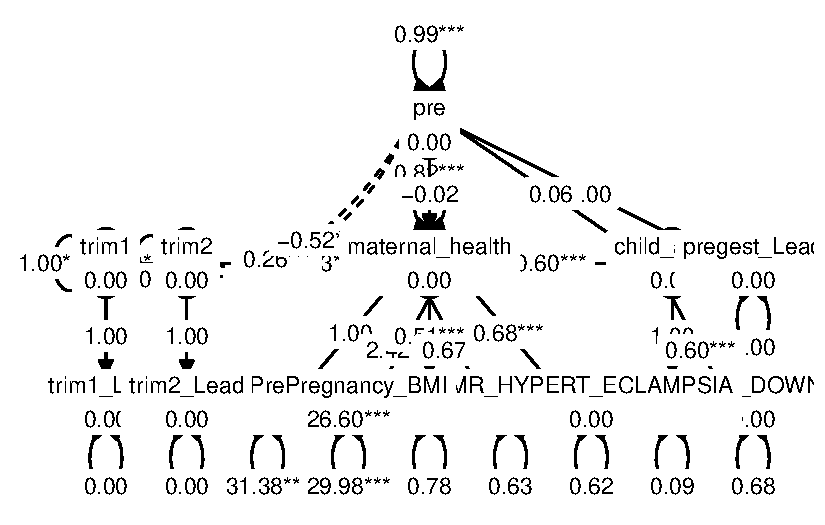
\includegraphics{analysis_files/figure-pdf/unnamed-chunk-5-1.pdf}

\hypertarget{discussion}{%
\section{Discussion}\label{discussion}}

The findings of this study highlight the importance of considering
maternal health factors when evaluating adverse pregnancy outcomes. The
positive associations observed between higher pre-pregnancy BMI,
diabetes, hypertensive disorders, and adverse pregnancy outcomes
highlight the significance of preconception and antenatal interventions
targeting these factors. Effective management of these maternal health
factors early in pregnancy may contribute to improved pregnancy outcomes
and mitigate the risks associated with adverse outcomes.

The application of latent variable analysis in this study offers a
robust framework for understanding the complex interrelationships among
maternal health factors and their impact on adverse pregnancy outcomes.
This approach allows for the simultaneous assessment of multiple
maternal health factors, as well as the identification of latent factors
that may be driving these associations. This information can be used to
develop more targeted and effective interventions to improve maternal
and fetal health.

In addition to the findings of this study, there is a growing body of
evidence that suggests that maternal health factors can also impact the
long-term health of the offspring. For example, maternal obesity has
been linked to an increased risk of childhood obesity, type 2 diabetes,
and cardiovascular disease. Therefore, it is important to consider the
long-term implications of maternal health factors when developing
interventions to improve pregnancy outcomes.

\hypertarget{conclusion}{%
\section{Conclusion}\label{conclusion}}

This study provides compelling evidence of the relationships between
maternal health factors and adverse pregnancy outcomes, specifically
chromosomal anomalies and Down syndrome in newborns. The results
emphasize the importance of considering the combined effects of maternal
age, pre-pregnancy BMI, diabetes, and hypertensive disorders on
pregnancy outcomes. Employing latent variable analysis offers a
comprehensive approach to studying the intricate associations between
maternal health factors and adverse pregnancy outcomes. By unraveling
these complex relationships, healthcare professionals can develop
targeted strategies to improve maternal and fetal health during
pregnancy.

Further research should delve deeper into the underlying mechanisms
linking these factors and explore potential interventions to mitigate
the risks associated with adverse pregnancy outcomes. Enhanced
understanding of these relationships will aid in developing personalized
and evidence-based strategies to optimize maternal and fetal health
outcomes.

Overall, the findings of this study suggest that maternal health factors
play a significant role in determining pregnancy outcomes. By
understanding these factors and their interactions, healthcare
professionals can develop targeted interventions to improve maternal and
fetal health.

\hypertarget{references}{%
\section*{References}\label{references}}
\addcontentsline{toc}{section}{References}

\hypertarget{refs}{}
\begin{CSLReferences}{0}{0}
\leavevmode\vadjust pre{\hypertarget{ref-R-base}{}}%
\CSLLeftMargin{1. }%
\CSLRightInline{R Core Team. R: A language and environment for
statistical computing {[}Internet{]}. Vienna, Austria: R Foundation for
Statistical Computing; 2023. Available from:
\url{https://www.R-project.org/}}

\leavevmode\vadjust pre{\hypertarget{ref-R-tidyverse}{}}%
\CSLLeftMargin{2. }%
\CSLRightInline{Wickham H. Tidyverse: Easily install and load the
tidyverse {[}Internet{]}. 2023. Available from:
\url{https://CRAN.R-project.org/package=tidyverse}}

\leavevmode\vadjust pre{\hypertarget{ref-tidyverse2019}{}}%
\CSLLeftMargin{3. }%
\CSLRightInline{Wickham H, Averick M, Bryan J, et al.
\href{https://doi.org/10.21105/joss.01686}{Welcome to the {tidyverse}}.
Journal of Open Source Software 2019;4(43):1686. }

\leavevmode\vadjust pre{\hypertarget{ref-R-rUM}{}}%
\CSLLeftMargin{4. }%
\CSLRightInline{Balise R, Odom G, Grealis K, Cardozo F. rUM: R templates
from the university of miami. 2023. }

\leavevmode\vadjust pre{\hypertarget{ref-R-table1}{}}%
\CSLLeftMargin{5. }%
\CSLRightInline{Rich B. table1: Tables of descriptive statistics in HTML
{[}Internet{]}. 2023. Available from:
\url{https://github.com/benjaminrich/table1}}

\end{CSLReferences}



\end{document}
